\documentclass{article}
\usepackage{enumitem}
\usepackage{mathtools}
\usepackage{fancyhdr}
\usepackage{xcolor}
\usepackage{mdframed}
\usepackage{bm}
\usepackage[letterpaper,portrait,left=2cm,right=2cm,top=3.5cm,bottom=2cm]{geometry}
\pagestyle{fancy}

\fancyhf{}
\rhead{Robert Wagner\\September 4, 2016}
\lhead{CISC 3220\\Assignment 1}
\newcounter{question}
\setcounter{question}{0}
\usepackage{amsmath,amsthm}
\usepackage{amssymb}
\usepackage{tikz}
\usetikzlibrary{arrows}
\usetikzlibrary{fit}


% magnitude bars
\newcommand{\norm}[1]{\lvert #1 \rvert}

% explicit vector
\newcommand{\Ve}[1]{\langle #1 \rangle}

% named vector
\newcommand{\Vn}[1]{\vec{#1}}

% a line with an arrow above
\newcommand{\Line}[1]{\overrightarrow{#1}}

% equals with question mark above
\newcommand{\?}{\stackrel{?}{=}}

% formatting for questions
\newcommand\Que[1]{%
   \leavevmode\noindent
   #1
}

% formatting for answers
\newcommand\Ans[2][]{%
   \leavevmode\noindent
   {
       \begin{mdframed}[backgroundcolor=blue!10]
       #2
       \end{mdframed}
   }
}

% this is like align but squashed     
\newenvironment{salign}
 {\par$\!\aligned}
 {\endaligned$\par}

% a matrix, parameter is column count
\newenvironment{Mat}[1]{%
  \left[\begin{array}{*{#1}{r}}
}{%
  \end{array}\right]
}


% a matrix, parameter is column count centered
\newenvironment{Cmat}[1]{%
  \left[\begin{array}{*{#1}{c}}
}{%
  \end{array}\right]
}

% an augmented matrix, with one augmented column
\newenvironment{Amat}[1]{%
  \left[\begin{array}{@{}*{#1}{r}|r@{}}
}{%
  \end{array}\right]
}
% an augmented matrix with n columns and n augmented columns
\newenvironment{Amat2}[1]{%
  \left[\begin{array}{@{~}*{#1}{r}| @{~~}*{#1}{r}}
}{%
  \end{array}\right]
}
% an augmented matrix with n columns and m augmented columns
\newenvironment{Amat3}[2]{%
  \left[\begin{array}{@{~}*{#1}{r}| @{~~}*{#2}{r}}
}{%
  \end{array}\right]
}


\begin{document}

\section{Exercises 1.1}
\begin{enumerate}
    \item Give a real-world example that requires sorting or a real-world example that requires computing a convex hull.
    \Ans{
    	Bank transaction database
    }
    %~\\
    \item Other than speed, what other measures of efficiency might we use in a real-world setting?
    \Ans{
        Minimize: Communcation data, programmer development time \\
        Maximize: User-friendliness
    }    
    %~\\
    \item Select a data structure you have used previously.  Describe its strengths and weaknesses.
    \Ans{
    	Linked List: \\
    	Strengths:  Dynamic size, Constant time insert + delete + concatenate \\
    	Weaknesses: Sequential (non-random) access, not-compact (pointer overhead) 
    }    
    %~\\
    \item How are the shortest path and traveling salesman problems similar?  How do they differ?
    \Ans{
    	Similar: They are both graph traversal optimization problems \\
    	Different: In the TS problem the begin and endpoint are fixed at the same point, In the SP problem the endpoints are free to vary.
    }
    %~\\
    \item Come up with a real-world problem in which only the best solution will do, then come up with a situation in which an approximation is enough.
    \Ans{ Best only: Wolfram-Alpha style algebraic solver \\
    	  Approximate: Almost all real-world problems ... Floating point error makes almost all computations approximate to some degree.
    }
\end{enumerate}

\section{Problem 1-1 Comparison of running times}
For each function $f(n)$\ and time $t$\ in the following table, determine the largest size $n$\ of a problem that can be solved in time $t$, assuming that the algorithm to solve the problem takes $f(n)$\ microseconds.
\Ans{
	\begin{tabular}{l|l|l|l|l|l|l|l}
		~      & 1s         & 1m & 1h & 1d & 1M & 1Y & 1C \\
		\hline
	$\log_2n$  & $10^{301030}$ & $6\times 10^{301031}$ & $3.6\times 10^{301033}$ & $8.6\times 10^{301034}$ & $2.6\times 10^{301036}$ & !!! & !!!   \\
	$\sqrt{n}$ & $10^{12}$  & $6.0\times 10^{13}$   & $3.6\times 10^{15}$   & $8.6\times 10^{16}$ & $2.6\times 10^{18}$   & $3.2\times 10^{19}$ & $3.2\times 10^{21}$\\
	$n$        & $10^6$     & $6.0\times 10^7$ & $3.6\times 10^9$ & $8.6\times 10^{10}$ & $2.6\times 10^{12}$ & $3.2\times 10^{13}$ & $3.2\times 10^{15}$ \\
	$n\log_2n$ & $6.4\times 10^4$& $3.8\times 10^6$ & $2.3\times 10^8$ & $5.5\times 10^9$ & $1.7\times 10^{11}$ & $2.0\times 10^{12}$ & $2.0\times 10^{14}$ \\
	$n^2$      & $1000$     & $6.0\times 10^4$ & $3.6\times 10^6$ & $8.6\times 10^7$ & $2.6\times 10^9$ & $3.2\times 10^{10}$ & $3.2\times 10^{12}$ \\
	$n^3$      & $100$      & $6.0\times 10^3$ & $3.6\times 10^5$ & $8.6\times 10^6$ & $2.6\times 10^8$ & $3.2\times 10^9$ & $3.2\times 10^{11}$ \\
	$2^n$      & $20$       & $1.2\times 10^3$ & $7.2\times 10^4$ & $1.7\times 10^6$ & $5.1\times 10^7$ & $6.2\times 10^8$ & $6.2\times 10^{10}$ \\
	$n!$       & $9$        & $540$ & $3.2\times 10^4$ & $7.7\times 10^5$ & $2.3\times 10^7$ & $2.8\times 10^8$ & $2.8\times 10^{10}$
	\end{tabular} 
}
\newpage
\section{Exercises 2.1}
\begin{enumerate}
	\item Using figure 2.2 as a model, illustrate the operation of insertion sort on the array $A = \Ve{31,41,59,26,41,58}$.
	\Ans{
	    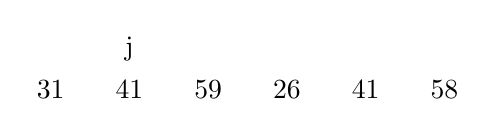
\begin{tikzpicture}
	        \node (31) {31};
	        \node[label={90:{j}}] (41) [right of=31]{41};
	        \node (59) [right of=41]{59};
	        \node (26) [right of=59]{26};
	        \node (41) [right of=26]{41};
	        \node (58) [right of=41]{58};
	    \end{tikzpicture} \\
	    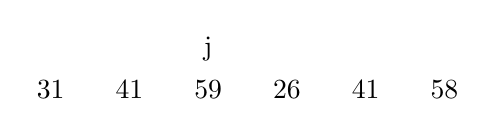
\begin{tikzpicture}
	        \node (31) {31};
	        \node (41) [right of=31]{41};
	        \node[label={90:{j}}] (59) [right of=41]{59};
	        \node (26) [right of=59]{26};
	        \node (41) [right of=26]{41};
	        \node (58) [right of=41]{58};
	    \end{tikzpicture} \\
	    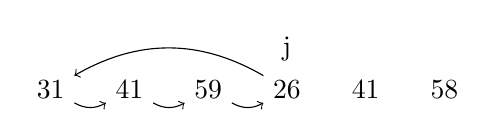
\begin{tikzpicture}
	        \node (31) {31};
	        \node (41a) [right of=31]{41};
	        \node (59) [right of=41a]{59};
	        \node[label={90:{j}}] (26) [right of=59]{26};
	        \node (41b) [right of=26]{41};
	        \node (58) [right of=41b]{58};
	        \draw[->] (26) to [bend right] (31);
	        \draw[->] (59) to [bend right] (26);
	        \draw[->] (41a) to [bend right] (59);
	        \draw[->] (31) to [bend right] (41a);
	     \end{tikzpicture} \\	
	     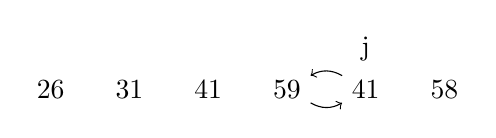
\begin{tikzpicture}
	         \node (26) {26};
	         \node (31) [right of=26]{31};
	         \node (41a) [right of=31]{41};
	         \node (59) [right of=41a]{59};
	         \node[label={90:{j}}] (41b) [right of=59]{41};
	         \node (58) [right of=41b]{58};
	         \draw[->] (41b) to [bend right] (59);
	         \draw[->] (59) to [bend right] (41b);
	     \end{tikzpicture} \\
	     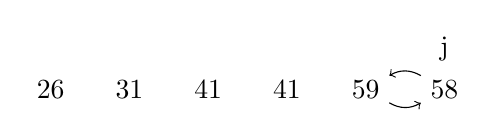
\begin{tikzpicture}
	         \node (26) {26};
	         \node (31) [right of=26]{31};
	         \node (41a) [right of=31]{41};
	         \node (41b) [right of=41a]{41};
	         \node (59) [right of=41b]{59};
	         \node[label={90:{j}}] (58) [right of=59]{58};
	         \draw[->] (58) to [bend right] (59);
	         \draw[->] (59) to [bend right] (58);
	     \end{tikzpicture} \\
	     Final sorted output:\\
	     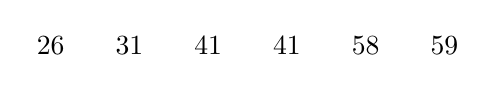
\begin{tikzpicture}
	         \node (26) {26};
	         \node (31) [right of=26]{31};
	         \node (41a) [right of=31]{41};
	         \node (41b) [right of=41a]{41};
	         \node (58) [right of=41b]{58};
	         \node (59) [right of=58]{59};
	     \end{tikzpicture} 
	     
	    
	}

	\item Rewrite the insertion sort to sort into non-ascending order instead of non-descending.
	\Ans{
		\setlength{\parindent}{5ex}
		\begin{tt}
		for j := 2 to A.length \\
		  \indent key := A[j] \\
		  \indent i := j - 1 \\
		  \indent while i > 0 and A[i] < key \\
		  \indent \indent A[i + 1] = A[i] \\
		  \indent \indent i := i - 1 \\
		  \indent A[i + 1] := key
		\end{tt}
	}
	\item Consider the searching problem. \\
	\setlength{\parindent}{10ex}
	        \indent input: a sequence of numbers $A = \Ve{a_1,a_2,\cdots,a_n}$\ and a value $v$. \\
	        \indent output: an index $i$\ such that $v=A[i]$\ or the special value NIL if $v \notin A$. \\
	 Write pseudo-code for linear search.  Use a loop invariant to prove your algorithm is correct.
	 \Ans{
	     \setlength{\parindent}{5ex}
	     \begin{tt}
	     	FIND(A, v) \\
	     	\indent for i := 1 to A.length \\
	     	\indent \indent if v = A[i] \\
	     	\indent \indent \indent return i \\
	     	\indent return NIL
	     \end{tt} \\
	     Loop invariant: for each index value $i$\ in the loop, we define a subset $A_i \subseteq A$\ such that $A_i = A[1\cdots i]$.  \\
	     Initial: At the beginning of each loop iteration, we know that $v \notin A_{i-1}$, where $A_0 = \emptyset$. \\
	     Maintenance: If $v=a_i$\ then we terminate the loop immediately. \\
	      Otherwise, since $A_i = A_{i-1} \cup \{a_i\}$, $v\notin A_{i-1}$\ and $v\notin \{a_i\}$\ it follows that $v \notin A_i$\ and the invariant holds.\\
	     Termination: Either the loop terminates when $v=a_i$\ invalidates the invariant, or when $i>A$.length.
	 }
	 \newpage
	 \item Consider the problem of adding two $n$-bit binary integers stored in two $n$-bit arrays $A$\ and $B$.  The sum of the two integers should be stored in binary form in an $(n+1)$\ element array $C$.  State the problem formally and write pseudo-code.
	 \Ans{
	 	There are two components to a binary sum:  Remainder term that keeps its current place (A XOR B) and a carried bit (A AND B) that is shifted to the next higher place (B SHL 1).  Loop invariant: $A + B = k$\ where $k$\ is constant. I actually return A here to cover the case where B=0 to start, since A + 0 = A.\\
	     \setlength{\parindent}{5ex}
	     \begin{tt}
	     	while B != 0 \\
	     	\indent C = A XOR B \\
	     	\indent B = (A AND B) SHL 1 \\
	     	\indent A = C \\
	     	return A	
	     \end{tt}
	 }
	 
\end{enumerate}

\section{Exercises 2.2}
\begin{enumerate}
	\item Express the function $\frac{n^3}{1000} - 100n^2 - 100n + 3$\ in terms of $\Theta$\ notation.
	\Ans{$\Theta(n^3)$}
	\item Consider sorting $n$\ numbers stored in array $A$\ by first finding the smallest element of $A$\ and exchanging it with the element in $A[1]$, then find the second smallest and exchange it with $A[2]$, and continue for the first $(n-1)$\ elements of $A$.  Write pseude-code for this algorithm known as selection sort.  Why does it need to run for only $(n-1)$\ elements?  Give best-case and worst-case running time on $\Theta$\ notation.
	\Ans{
	  \setlength{\parindent}{5ex}
	  \begin{tt}
	  	for i := 1 to n-1 \\
	  	\indent key := A[i] \\
	  	\indent index := i \\
	  	\indent for j := i + 1 to n \\
	  	\indent \indent if A[j] < key \\
	  	\indent \indent \indent key := A[j] \\
	  	\indent \indent \indent index := j \\
	  	\indent A[index] := A[i] \\
	  	\indent A[i] := key
	  \end{tt} \\
	  Selection sort outer loop only runs to $(n-1)$\ since the loop invariant guarantees that all elements in the subarray $A^\prime[1\cdots i]$\ are less than all elements in the subarray $A[i+1\cdots n]$.  Thus when the $(n-1)$\ iteration has terminated, the element $A[n] \geq A^\prime[k]$\ for all $k \in \{1\cdots n-1\}$, which means an $n$th iteration of the outer loop is unnecessary. \\
	  Worst-case time: $\Theta(n^2)$, 
	  Best-case time: $\Theta(n^2)$.
	}
	\item Consider linear search again.  How many elements of the input sequence need to be checked on the average, assuming that the element being searched for is equally likely to be any element in the array?  How about in the worst case?  What are the average-case and worst-case running times?  Justify your answer.
	\Ans{On average we need to check $n/2$\ elements, and in the worst case we need to check all $n$\ elements.  The running time is thus $\Theta(n/2)$\ in the average case and $\Theta(n)$\ in the worst case.}
	\item How can we modify almost any algorithm to have a good best-case running time?
	\Ans{By tailoring the algorithm to optimize the most frequently encountered input set, and short-circuiting execution by testing for best-case input and returning early.}
\end{enumerate}
\section{Exercises 2.3}
\begin{enumerate}
	\item Using figure 2.4 as a model, illustrate the operation of merge sort on array $A=\Ve{3,41,52,26,38,57,9,49}$.
	\Ans{
	 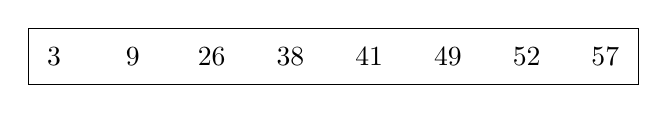
\begin{tikzpicture}
	 \node (3) {3};
	 \node (9) [right of=3]{9};
	 \node (26) [right of=9]{26};
	 \node (38) [right of=26]{38};
	 \node (41) [right of=38]{41};
	 \node (49) [right of=41]{49};
	 \node (52) [right of=49]{52};
	 \node (57) [right of=52]{57};
	 \node[draw,fit=(3)(57)] (box){};
	 \end{tikzpicture} ~ Final sorted array \\
	 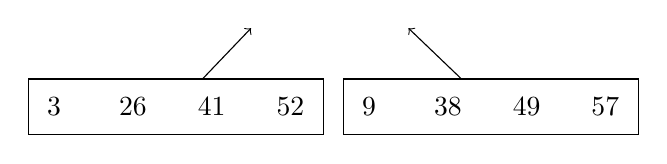
\begin{tikzpicture}
	 \node (3) {3};
	 \node (26) [right of=3]{26};
	 \node (41) [right of=26]{41};
	 \node (52) [right of=41]{52};
	 \node (9) [right of=52]{9};
	 \node (38) [right of=9]{38};
	 \node (49) [right of=38]{49};
	 \node (57) [right of=49]{57};
	 \node[draw,fit=(3)(52)] (box1){};
	 \node[draw,fit=(9)(57)] (box2){};
	 \draw[->] (box1) -- (2.5,1);
	 \draw[->] (box2) -- (4.5,1);
	 \end{tikzpicture} \\
	 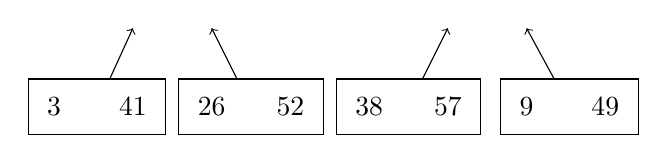
\begin{tikzpicture}
	 \node (3) {3};
	 \node (41) [right of=3]{41};
	 \node (26) [right of=41]{26};
	 \node (52) [right of=26]{52};
	 \node (38) [right of=52]{38};
	 \node (57) [right of=38]{57};
	 \node (9)  [right of=57]{9};
	 \node (49) [right of=9]{49};
	 \node[draw,fit=(3)(41)] (box1){};
	 \node[draw,fit=(26)(52)] (box2){};
	 \node[draw,fit=(38)(57)] (box3){};
	 \node[draw,fit=(9)(49)] (box4){};
	 \draw[->] (box1) -- (1,1);
	 \draw[->] (box2) -- (2,1);
	 \draw[->] (box3) -- (5,1);
	 \draw[->] (box4) -- (6,1);
	 \end{tikzpicture} \\
	 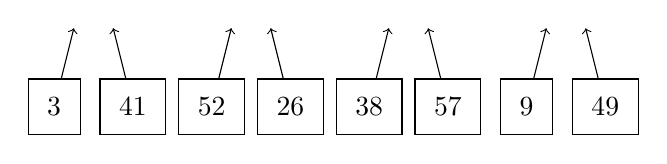
\begin{tikzpicture}
	 \node (3) {3};
	 \node (41) [right of=3]{41};
	 \node (52) [right of=41]{52};
	 \node (26) [right of=52]{26};
	 \node (38) [right of=26]{38};
	 \node (57) [right of=38]{57};
	 \node (9)  [right of=57]{9};
	 \node (49) [right of=9]{49};
	 \node[draw,fit=(3)] (box1){};
	 \node[draw,fit=(41)] (box2){};
	 \node[draw,fit=(52)] (box3){};
	 \node[draw,fit=(26)] (box4){};
	 \node[draw,fit=(38)] (box5){};
	 \node[draw,fit=(57)] (box6){};
	 \node[draw,fit=(9)]  (box7){};
	 \node[draw,fit=(49)] (box8){};
	 \draw[->] (box1) -- (0.25,1);
	 \draw[->] (box2) -- (0.75,1);
	 \draw[->] (box3) -- (2.25,1);
	 \draw[->] (box4) -- (2.75,1);
	 \draw[->] (box5) -- (4.25,1);
	 \draw[->] (box6) -- (4.75,1);
	 \draw[->] (box7) -- (6.25,1);
	 \draw[->] (box8) -- (6.75,1);
	 \end{tikzpicture} ~ Initial unsorted array
	}
	\item Rewrite the merge procedure so that it does not use sentinels, instead stopping once either array $L$\ or $R$\ has had all elements copied back to $A$\ and then copying the remainder of the other back to $A$.
	\Ans{
	    \setlength{\parindent}{5ex}
	    \begin{tt}
	    	MERGE(A, p, q, r) \\
	    	\indent n1 := q - p + 1 \\
	    	\indent n2 := r - q \\
	    	\indent let L[1 .. n1] and R[1 .. n2] be new arrays \\
	    	\indent for i := 1 to n1 \\
	    	\indent \indent L[i] := A[p + i - 1] \\
	    	\indent for j := 1 to n2 \\
	    	\indent \indent R[j] := A[q + j] \\
	    	\indent i := j := 1 \\
	    	\indent k := p \\
	    	\indent while k <= p and i <= n1 and j <= n2 \\
	    	\indent \indent if L[i] <= R[j] \\
	    	\indent \indent \indent A[k++] := L[i++] \\
	    	\indent \indent else A[k++] := R[j++] \\
	    	\indent while i <= n1 \\
	    	\indent \indent A[k++] := L[i++] \\
	    	\indent while j <= n2 \\
	    	\indent \indent A[k++] := R[j++] \\
	    \end{tt}
	    	
	}
	\item Use mathematical induction to show that when $n$\ is an exact power of 2, then the solution of the recurrence
	\[
		T(n) = \begin{cases}
	                   2 & \text{if } n=2 \\
	           2T(n/2)+n & \text{if } n=2^k, k>1
	        \end{cases}
	\]
	is $T(n)=n\log_2 n$.
	\Ans{
	    \begin{align*}
	    \shortintertext{Base Case: Let $k=1$, thus}
	        n &= 2^k = 2^1 = 2\\
	        T(2^k)&=T(2)=2\log_22 = (2)(1) = 2 \checkmark
	    \shortintertext{Inductive Step: Let $k > 1$, and suppose $n=2^k$.  Note that} 
	    n/2 &= 2^{k-1} \\ 
	    T(n/2) &= T(2^{k-1}) \\
	    k &= \log_2n
	    \shortintertext{Assume $
	    T(2^{k-1}) = 2^{k-1}\log_22^{k-1}$\ is true.  Then}
	    T(2^k) &= T(n) = 2(2^{k-1}\log_22^{k-1}) + 2^k \\
	    \shortintertext{Which simplifies to}
	    T(2^k) &= T(n) = (2^k)(k-1+1) = (2^k)(k)\\
	           &= n\log_2n
	    \end{align*}
	    Thus we have shown that the inductive step holds and the recurrence is true for all $k > 1$. \qed
	}
	\item We can express insertion sort as a recursive procedure as follows: \\
	In order to sort $A[1\cdots n]$, we recursively sort $A[1\cdots n-1]$\ and then insert $A[n]$\ into the sorted array \\ $A[1\cdots n-1]$.  Write a recurrence for the running time of this recursive version of insertion sort.
	\Ans{
		\[T(n) = \begin{cases} \Theta(1) & \text{if } n=1 \\ T(n-1) + \Theta(n) & \text{if } n>1
		         \end{cases}\]
	  Where $T(n-1)$\ term refers to the recursive sort $A[1..n-1]$\ and $\Theta(n)$\ refers to the time to insert $A[n]$\ into the sorted array.	
	}
	\item Referring back to the searching problem, observe that if the sequence $A$\ is sorted, we can check the midpoint of the sequence against $v$\ and eliminate half the sequence from consideration.  The binary search algorithm repeats this procedure, halving the size of the remaining portions of the sequence each time.  Write pseude-code for binary search.  Argue that the worst-case running time is $\Theta(\log_2 n)$.
	\Ans{
	  \setlength{\parindent}{5ex}
	  \begin{tt}
	  	BSEARCH(A, l, r, v) \\
	  	\indent mid := l + (l - r) / 2 \\
	  	\indent if A[mid] = v \\
	  	\indent \indent return mid \\
	  	\indent if mid = l \\
	  	\indent \indent return NIL \\
	  	\indent if v < A[mid] \\
	  	\indent \indent return BSEARCH(A, l, mid - 1, v) \\
	  	\indent else \\
	  	\indent \indent return BSEARCH(A, mid + 1, r, v)
	  \end{tt}	\\~\\
	  Note that on each recursive iteration, we discard half of the previous iteration set.  Thus our worst-case recurrence is
	  \[
	     T(n)=\begin{cases} \Theta(1) & \text{if }n=1\\
	                        T(n/2) + \Theta(1) & \text{if }n>1 \end{cases}
	  \]
	  Which can be shown to be $T(n) = \log_2n$\ by the recursion tree method.  Thus the worst-case running time is $\Theta(\log_2n)$.
	}
	\newpage
	\item Observe that the while loop of lines 5-7 of the insertion sort procedure in section 2.1 uses a linear search to scan backwards through the sorted sub-array.  Can we use a binary search to improve the worst-case running time to $\Theta(n\log_2 n)$?
	\Ans{NO, using the binary search will not improve the worst-case time since the algorithm has to insert the $a_j$\ element into its place in the already sorted $A_{j-1}$\ subarray, which requires $\Theta(j-1)$\ worst-case time per iteration of $j$, which sums to $\Theta(n^2) >> \Theta(n\log_2n)$.}
	\item Describe an $\Theta(n\log_2n)$\ algorithm that, given a set $S$\ of $n$\ integers, and another integer $x$, determines whether there exists two numbers in $S$\ whose sum is $x$.
	\Ans{
		First, Sort the set $S$\ into an ordered list $S^\prime$\ which requires $\Theta(n\log_2n)$\ worst-case time.\\
		Second, Iterate through $S^\prime$\ where $i=1\cdots n-1$\ indexes the element $s^\prime_i$. \\
		On each iteration, do a binary search through the subarray of $S^\prime$\ to the right of the current index for a value $v=x - S^\prime[i]$.  If the value is found we have fulfilled our test and can terminate the loop.  This process requires $n$\ iterations of $\Theta(\log_2n) = \Theta(n\log_2n)$ in the worst case. \\
		Thus the worst-case time is $\Theta(n\log_2n) + \Theta(n\log_2n) = \Theta(n\log_2n)$.
		}
\end{enumerate} 
\section{Problem 2-1 Insertion sort on small arrays in merge sort}
    Although merge sort runs in $\Theta(n\log_2n)$\ worst-case time and insertion sort runs in $\Theta(n^2)$\ worst-case time, the constant factors in insertion sort can make it faster in practice for small problem sizes on many machines.  Consider a modification of merge sort in which $n/k$\ sublists of length $k$\ are sorted using insertion sort and then merged using the standard merge mechanism, where $k$\ is a value to be determined.
    \begin{enumerate}
    	\item Show that insertion sort can sort the $n/k$\ sublists, each of length $k$, in $\Theta(nk)$\ worst-case time.
    	\Ans{For each of the sublists, the size is $k$\ thus the worst-case running time of insertion sort is $\Theta(k^2)$\ per sublist. Since there are $n/k$\ of them, the total worst-case time is $(n/k)\Theta(k^2)$\ which cancels out to $\Theta(nk)$. }
    	\item Show how to merge the sublists in $\Theta(n\log_2(n/k))$\ worst-case time.
    	\Ans{
    	   \begin{salign} 
    	   	  T(n) = \begin{cases}
    	                \Theta(k) & \text{if } n\leq k\\
    	                2T(n/2) + \Theta(1) & \text{if } n > k
    	            \end{cases} 
    	   \shortintertext{Since the recurrence stops when $n=k$, this results in}
    	     T(n) = [(n/k)\Theta(k)]\times[\Theta(log_2n)-\Theta(log_2k)] = \Theta(n\log_2(n/k)) 
    	  \end{salign}  	
    	}
    	\item Given that the modified algorithm runs in $\Theta(nk + n\log_2(n/k))$\ worst-case time, what is the largest value of $k$\ as a function of $n $\ for which the modified algorithm has the same running time as standard merge sort?
    	\Ans{\centering
    		\begin{salign}
    		    \Theta(nk+\log_2(n/k)) &\leq \Theta(n\log_2n) \\
    		    nk+log_2n-log_2k &\leq nlog_2n \\
    		    nk-log_2k &\leq (n-1)log_2n \\
    		    k &\leq \frac{n-1}{n}\log_2n + C
    		\end{salign}
    	}
    	\item How should we choose $k$\ in practice?
    	\Ans{Suppose $n=2^x$\ for some $x\in \mathbb{R}$.
    		Let $k=\lfloor x\rfloor$.  This is easy to calculate and guarantees that $k \leq \log_2n$. 
    	}
    \end{enumerate}
\section{Problem 2-2 Correctness of Bubblesort}
    Bubblesort is a popular, but inefficient, sorting algorithm.  It works by repeatedly swapping adjacent elements that are out of order.\\
    \setlength{\parindent}{5ex}
    
    \begin{tt}
    	\indent BUBBLESORT(A)\\
    	\indent 1\indent for i := 1 to A.length - 1\\
    	\indent 2\indent \indent for j := A.length downto i + 1 \\
    	\indent 3\indent \indent \indent if A[j] < A[j-1] \\
    	\indent 4\indent \indent \indent \indent exchange A[j] with A[j-1]
    \end{tt} \\
    \begin{enumerate}
    	\item Let $A^\prime$\ denote the output of BUBBLESORT(A).  To prove that BUBBLESORT is correct, we need to prove that it terminates and that 
    	\[A^\prime[1] \leq A^\prime[2] \leq \cdots \leq A^\prime[n] \]
    	where $n = A.$length.  In order to show that BUBBLESORT actually sorts, what else do we need to prove?
    	\Ans{That $A^\prime$\ is a permutation of $A$, i.e. we can define a bijection $f:A\to A^\prime$. }
    	\item State precisely a loop invariant for the for loop in lines 2-4, and prove that this loop invariant holds.  Your proof should use the structure of the loop invariant proof presented in this chapter.
    	\Ans{
    		Loop invariant: the lowest value element of subarray $S=A[j\cdots n]$\ (where $n=A.$length) is $A[j]$.\\
    		Initialization:  On first iteration $j=n$\ so $S$\ has a single element and $A[j]$\ is the lowest value trivially. \\
    		Maintenance: On each iteration, if $A[j-1]$\ is a lower value than $A[j]$\ then they are exchaged, so that the loop invariant holds for the next iteration when $j$ is decremented. \\
    		Termination: The loop terminates when $j=i+1$, and the loop invariant guarantees that $A[i]$\ is the lowest value element of the subarray $A[i\cdots n]$, i.e. $A[i] \leq A[k]$\ for all $k\in \{i+1\cdots n\}$.
    	}
    	\item Using the termination condition of the loop invariant proved in part (b), state a loop invariant for the for loop in lines 1-4 that will allow you to prove the inequality above.
    	\Ans{
    		Loop invariant: The subarray $T=A^\prime[1\cdots i]$\ is sorted, i.e. $A^\prime[1]\leq \cdots \leq A^\prime[i]$.\\
    	    Initialization: On first iteration $i=1$\ so $T$\ has a single element and is sorted trivially. \\
    	    Maintenance: On each iteration, The inner loop guarantees $A^\prime[i]$\ is less than or equal to all elements that follow.  Thus all elements before $i$\ were the lowest value of the subarray on their respective iteration, and thus the invariant holds. \\
    	    Termination: The loop terminates when the subarray has one element, and the array is sorted. }
    	\item What is the worst-case running time of bubblesort?  how does it compare to the running time of insertion sort?
    	\Ans{The worst case running time is $\Theta(n^2)$\ which is identical to the worst case of Insertion sort. In practice however insertion sort is faster than bubble sort since it executes far fewer exchanges in the average case, even though it executes a similar number of compares.}
    \end{enumerate}
    \newpage
\section{Problem 2-3 Correctness of Horner's Rule}
    The following code fragment implements Horner's rule for evaluating a polynomial
    \begin{align*}
        P(x) &= \sum_{k=0}^n a_kx^k \\
             &= a_0 + x(a_1 + x(a_2 + \cdots + x(a_{n-1} + xa_n)\cdots))
    \end{align*}
    Given the coefficients $a_0, a_1, \cdots a_n$\ and a value for $x$:
    \begin{verbatim}
    y = 0
    for i = n downto 0
        y = a_i + xy
    \end{verbatim}
    \begin{enumerate}
    	\item In terms of $\Theta$-notation, what is the running time of this code fragment for Horner's rule?
    	\Ans{$\Theta(n+1)$\ where $n$\ is the degree of the polynomial.}
    	\item Write pseudo-code to implement the naive polynomial evaluation algorithm that computes each term of the polynomial from scratch. What is the running time of this algorithm?  How does it compare to Horner's rule?
    	\Ans{
    	   \setlength{\parindent}{5ex}
    	   \begin{tt}
    	   	total := 0 \\
    	   	for k := 1 to n \\
    	   	\indent term := A[k] \\
    	   	\indent for j := 1 to k \\
    	   	\indent \indent term := term * x \\
    	   	\indent total := total + term \\
    	   	return total
    	   	\end{tt} \\
    	   	The worst-case running time of this algorithm is $\Theta\left(\frac{n(n+1)}{2}\right) = \Theta(n^2)$, which is worse than Horner's. 
    	}
    	\item Consider the following loop invariant: \\
    	At the start of each iteration of the for loop of lines 2-3,
    	\[
    	    y = \sum_{k=0}^{n-(i+1)} a_{k+i+1} x^k
    	\]
    	Interpret a summation with no terms equalling 0.  Following the structure of the loop invariant proof presented in this chapter, use the loop invariant to show that, at termination, 
    	\[
    	    y = \sum_{k=0}^n a_k x^k
    	\]
    	\Ans{
    		\begin{align*}
    		\shortintertext{Initialization: before the first iteration}
    		y &= 0 = \sum_{k=0}^{-1}a_{n+1}x^0
    		\shortintertext{since the sum bounds are invalid, the result is $0$\ which is consistent.}
    		\shortintertext{Maintenance:} 
    			y^\prime &= a_i + xy = a_ix^0 + \sum_{k=0}^{n-i-1}a_{k+i+1}x^{k+1}
    		\shortintertext{If we define $k^\prime = k+1$\ and $i^\prime=i-1$, then} 
    		    y^\prime &= a_ix^0 + \sum_{k^\prime=1}^{n-(i^\prime+1)}a_{k^\prime+(i^\prime+1)}x^{k^\prime}
    		\shortintertext{We can combine the $a_ix^0$\ term into the sum as a $k^\prime=0$ term}
    		    y^\prime &= \sum_{k^\prime=0}^{n-(i^\prime+1)}a_{k^\prime+i^\prime+1}x^{k^\prime}
    		\shortintertext{Which maintains the loop invariant for the next iteration since $i$\ is decremented each iteration.}
    		\shortintertext{Termination: At the termination of our final iteration, $i^\prime=-1$\ and}
    		   y^\prime &= \sum_{k^\prime=0}^{n-(-1+1)}a_{k^\prime+1-1}x^{k^\prime}
    		             = \sum_{k=0}^{n}a_kx^k
    		\end{align*}
    	}
    	\item Conclude by arguing that the given code fragment correctly evaluates a polynomial characterized by coefficients $a_0, a_1, \cdots, a_n$.
    	\Ans{
    	    We have shown that a loop invariant is maintained which terminates in a state where the value \\ 
    	    $y=\sum_{k=0}^na_kx^k$\ which is the value a polynomial with coefficients $a_0,a_1,\cdots,a_n$\ evaluates to.  \\
    	    Thus the code fragment correctly evaluates a polynomial of finite degree.
    	}
    \end{enumerate}
\end{document}  